% !TEX root = tarasov-qasp-zh.tex
% 章首扉图与格言（sec-09，分子物理学）在英文源 ch-17.tex 尾部（有效代码），归 zh/ch-17-zh.tex；
% 本章文件首尾均无有效 sec 块（ch-18.tex 尾部那组 sec 块为 % 注释的死代码副本，未搬入）。

\chapter[你对物质的分子动理论了解多少？]{你对物质的分子动理论了解多少？\label{ch-18}}

\begin{dialogue}

\tchr 常见的考题之一是：\hlred{物质分子动理论的基本原理有哪些？}这个问题你会怎样回答？

\stda 我会说出两条基本原理。第一，一切物体都由分子组成；第二，分子处于无规则的热运动状态。

\tchr 你的回答很典型：简短，却相当不完整。我注意到，学生对这个问题通常抱着应付的态度。他们多半不知道关于分子动理论的基本原理究竟应该说些什么，只用几句泛泛的话搪塞过去。因此，我觉得有必要比较详细地讨论一下物质的分子动理论（molecular-kinetic theory of matter）。我先列出可以视为这一理论之基本原理的几条内容。
\begin{enumerate}[label=\arabic*.,leftmargin=1cm]
\item 物质具有“颗粒性”结构：它由分子（或原子）组成。1 克分子（gram-molecule）物质含有 $N_{A} = \num{6d23}$ 个分子，与物质所处的物态无关（数 $N_{A}$ 称为阿伏加德罗常数，Avogadro's number）。
\item 物质的分子处于不停息的热运动之中。
\item 分子热运动的性质取决于分子间相互作用的性质，并且当物质从一种物态过渡到另一种物态时发生改变。
\item 分子热运动的剧烈程度取决于物体被加热的程度，后者由绝对温度（absolute temperature）$T$ 表征。理论证明，单个分子的平均能量 $e$ 与温度 $T$ 成正比。例如，对于单原子（single-atom）分子，有
\begin{equation}%
e = \frac{3}{2} kT
\label{eq-98}
\end{equation}
其中 $k= \num{1.38d-16}$ erg/deg 是一个物理常量，叫做玻耳兹曼常量（Boltzmann's constant）。

\item 从分子动理论的观点看，物体的总能量 $E$ 是下列各项之和：
\begin{equation}%
E = E_{k} + E_{p} + U
\label{eq-99}
\end{equation}
其中 $E_{k}$ 是物体整体运动的动能，$E_{p}$ 是物体整体在某个外场中的势能，$U$ 是与物体内分子热运动相联系的能量。能量 $U$ 称为物体的内能（internal energy）。在处理各种能量平衡问题时把内能包括进来，是分子动理论的一个特征。
\end{enumerate}
\pnote{原书给出的两个常数均只取两位有效数字。按 2019 年 SI 单位制改革，阿伏加德罗常数取定义值 $N_{A}=6.02214076\times 10^{23}\ \mathrm{mol^{-1}}$（以此定义摩尔），玻耳兹曼常量取定义值 $k=1.380649\times 10^{-23}\ \mathrm{J/K}$（以此定义开尔文）。原书的 $k$ 用 CGS 单位：$1~\mathrm{erg}=10^{-7}~\mathrm{J}$，故 $\num{1.38d-16}$ erg/deg 即 $1.38\times 10^{-23}$ J/K，与定义值一致到三位。位数的差异不影响任何中学结论与数量级估算（下文估算铁原子间距用的就是 $6\times 10^{23}$）。}
\pnote{这五条原理对应人教版选择性必修第三册第一章《分子动理论》：第 1 节“分子动理论的基本内容”与第 2 节油膜法实验对应第 1、2 条；第 3 节给出“温度是分子平均动能的标志”，即式~\eqref{eq-98} 的定性形式；第 4 节“分子动能和分子势能”定义内能为物体内所有分子热运动动能与势能之和，即式~\eqref{eq-99} 的 $U$。原书把整体动能 $E_{k}$、整体势能 $E_{p}$ 与内能 $U$ 并列为物体总能量的三个部分，正对应中学“机械能与内能”之分。}

\stdb 我们习惯上认为，克分子和阿伏加德罗常数是化学里的东西。
\\
\tchr 大概正因为如此，参加物理考试的学生常常不知道什么是克分子，而且照例总是确信阿伏加德罗常数只与气体有关。请记住：\hlblue{克分子是克数在数值上等于其分子量的那部分物质（而绝不是像某些学生所说的那样，是用克表示的一个分子的重量）；克原子（gram-atom）是克数在数值上等于其原子量的那部分物质；阿伏加德罗常数则是任何物质的一个克分子（或一个克原子）中所含的分子数（或原子数），与该物质处于何种物态无关。}

我想指出，阿伏加德罗常数是沟通物质宏观特性与微观特性的一座桥梁。例如，利用它可以把物质的一个微观特性——分子（或原子）间的平均距离——用密度和分子量（或原子量）表示出来。比如取固态铁：它的密度是
$\rho=\SI{7.8}{\gram\per\cubic\centi\metre}$，原子量 $A =56$。我们来求铁中原子间的平均距离。步骤如下：在 $A\,\, \si{\gram}$ 铁中有 $N_A$ 个原子，那么在 \SI{1}{\gram} 铁中就应有 $N_{A}/A$ 个原子。由此可知，\SI{1}{\cubic\centi\meter} 中有 $\rho N_{A}/A$ 个原子。于是，铁的每个原子平均占有 $A/\rho N_{A} \si{\cubic\centi\meter}$ 的体积。所求的原子间平均距离近似等于这个体积的立方根
\begin{equation*}%
x \approx \sqrt[3]{\frac{A}{\rho N_{A}}} =\sqrt[3]{\frac{56}{7.8\times \num{6d23}}} \,\, \si{\centi\meter} \approx \num{2d-8}\,\, \si{\centi\meter}
\end{equation*}
\pnote{克分子、克原子是苏联教材时代的计量术语；1971 年 SI 将“摩尔”（mole，符号 mol）定为物质的量的基本单位后，现行课程一律用摩尔计量：1 克分子即 1 mol 物质，含阿伏加德罗常数个分子（人教版高中化学必修第一册引入物质的量）。相应地，原书的分子量／原子量现称相对分子质量／相对原子质量，数值不变。原书强调的易错点——克分子不是“一个分子的克重量”——改用摩尔表述后同样值得警惕。}
\pnote{由宏观量（密度、原子量、阿伏加德罗常数）估算微观量（原子间距、分子大小）是中国教材与高考的经典题型，与人教版选择性必修第三册第一章第 2 节“实验：用油膜法估测油酸分子的大小”同类：那里用一滴油酸的体积除以单分子油膜的面积，这里对每个原子占据的体积开立方。所得 $\num{2d-8}$ cm 即 $2\times 10^{-10}$ m（0.2 nm），与公认的分子线度量级 $10^{-10}$ m 一致。}

\stdb 您刚才说，分子热运动的性质取决于分子间的相互作用，并且在从一种物态过渡到另一种物态时发生改变。请您更详细地解释一下。

\begin{figure}[!h]%
\centering
%\fbox{
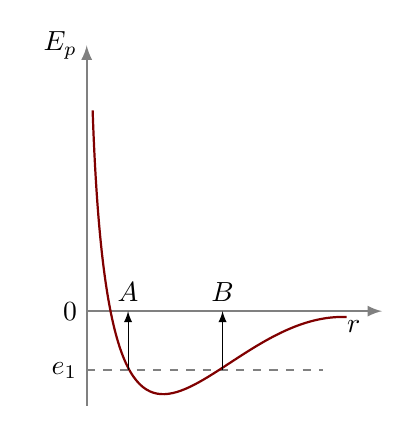
\begin{tikzpicture}[>=latex,scale=.75]
\clip (-1,-1.6) rectangle (5, 4.8);
\draw[thick, ->,gray] (0,0) -- (5,0);
\draw[thick, ->,gray] (0,-1.8) -- (0,4.5);
\draw[thick, dashed,gray] (0,-1) -- (4,-1);
\node [left] at (0,4.5) {$E_{p}$};
\node [left] at (0,-1) {$e_{1}$};
\node [below left] at (4.8,0) {$r$};
\node [left] at (0,0) {0};
\draw[ thick,Maroon] (0.1,3.4) .. controls (.38,-4.8) and (2.,0.).. (4.4, -0.1);
\draw[<-] (.7,0) -- (.7,-1);
\node [above] at (0.7,0) {$A$};
\draw[<-] (2.3,0) -- (2.3,-1);
\node [above] at (2.3,0) {$B$};
%\draw[gray,step=0.25] (-0.6,-3) grid (5, 5.3);
\end{tikzpicture}%}
\caption[分子间相互作用势能与分子间距离的关系。]{分子相互作用势能 $E_{p}$ 随两分子中心间距离 $r$ 的变化关系。\label{fig-69}}
\end{figure}

\tchr 定性地看，两个分子的相互作用可以用\figr{fig-69} 所示的曲线来描述。这条曲线表示分子相互作用的势能 $E_{p}$ 随两分子中心间距离 $r$ 的变化。当分子间距离足够大时，曲线 $E_{p}(r)$ 渐近地趋于零，也就是说，分子实际上不再相互作用。当分子互相靠近时，曲线 $E_{p}(r)$ 转而向下。随后，当它们彼此靠得足够近时，分子开始互相排斥，曲线 $E_{p}(r)$ 转而向上，$E_{p}$ 继续增大（这种排斥意味着分子不能自由地彼此穿透）。可以看出，$E_{p}(r)$ 曲线有一个特征性的极小值。

\stdb 什么是负能量？

\tchr 我们知道，能量可以从任意一个基准起算。比如，石块的势能可以从当地的地面算起，也可以从海平面算起，这毫无分别。在我们这个情形里，零点对应于相距无穷远的两个分子之间的相互作用能。因此，分子的能量为负，意味着它处于束缚态（bound state，与另一个分子束缚在一起）。要把这个分子“释放”出来，必须给它添一些能量，把它的能量提高到零水平。设分子的能量为负值 $e_{1}$（见\figr{fig-69}）。由曲线显然可见，在这种情形下，分子离它的邻居不能比点 $B$ 更远，也不能比点 $A$ 更近。换句话说，分子将在邻近分子的场中于点 $A$ 与 $B$ 之间振动（更准确地说，是组成束缚系统的两个分子作相对振动）。
\pnote{分子间相互作用的图像见人教版选择性必修第三册第一章“分子间的作用力”部分：引力与斥力同时存在、都随距离增大而减小，斥力减小得更快，平衡位置处合力为零——对应本图势能曲线的最低点（平衡距离 $r_{0}$ 的量级为 $10^{-10}$ m）。分子在势阱中于最低点附近往复，正是晶体、液体中分子热振动的图像。“能量为负即束缚态”与力学中“束缚系统总机械能为负”（如绕地运行的卫星）同构：要脱离束缚，必须补足能量到零。}

在气体中，分子彼此的平均距离如此之大，以致可以认为它们实际上不相互作用。每个分子都自由飞行，只是比较少地发生碰撞。每个分子都参与三种运动：平动、转动（分子绕自身轴转动）和振动（分子内的原子彼此相对振动）。若是单原子分子，就只有平动。

在晶体中，分子靠得如此之近，以致形成一个统一的束缚系统。这时，每个分子都在由整个分子集体的相互作用所建立的某种总的力场中振动。晶体作为分子的共同束缚系统，其特征是存在有序的三维结构——晶格（crystal lattice）。晶格的结点就是各个分子的平衡位置，分子绕这些位置完成复杂的振动运动。应当指出，在某些情形下，分子形成晶体时仍在一定程度上保持自己的个性。这时要区分分子在晶体场中的振动与各个分子内部原子的振动。这种情形出现在分子内原子的结合能显著高于分子自身在晶格中的结合能的时候。但在大多数情形下，分子形成晶体时并不保持自己的个性，结果晶体不是由一个个分子组成，而是由一个个原子组成。显然，这时没有分子内部的振动，只有原子在晶体场中的振动。关于物质中原子和分子的热运动，考生应当掌握的最低限度的知识就是这些。通常，考生谈到物质中热运动的性质时，说到“无规则运动”就再也讲不下去了，想以此掩盖自己关于热运动更详细知识的缺乏。

\stdb 可您还一点也没讲液体中分子热运动的性质呢。

\tchr 液体中的热运动比其他物质中的更复杂。液体占据着气体与晶体之间的中间位置：它既表现出粒子间强烈的相互作用，又在结构上表现出相当程度的无序。研究晶体的困难在于粒子相互作用强，这在很大程度上被有序结构——晶格——的存在所补偿；研究气体的困难在于各粒子位置无序，这被粒子间实际上完全不存在相互作用所补偿。而液体兼有上述两种困难，却没有相应的补偿因素。可以说，在液体中，分子照例完全保持着自身的个性。液体中的运动五花八门：分子的移动、分子的转动、分子内原子的振动，以及分子在邻近分子场中的振动。最麻烦的是，严格说来，所有这些类型的运动都不能分开来（也就是不能“以纯粹的形式”）处理，因为各种运动之间存在强烈的相互影响。

\stdb 我不明白，分子的平动怎么能够同它在邻近分子场中的振动结合在一起。

\tchr 人们提出过种种试图把这两种运动结合起来的模型。例如，其中一个模型假定分子的行为如下：它在邻近分子所建立的场中振动一段时间，然后跳一下，进入新的环境，在新环境中振动，再跳一下，如此等等。这样的模型称为“跳跃扩散模型”（jump-diffusion model）。

\stdb 看来，原子在晶体中的扩散正是这样进行的。

\tchr 对。只是要记住，在晶体中这一过程更慢：跳入新环境的次数要少得多。还有另一种模型，按这种模型，液体中分子的行为是：它在周围分子的环绕中振动，而整个环境在空间中平缓地移动（“漂移”）并逐渐变形。这称为“连续扩散模型”（continuous-diffusion model）。

\stdb 您说过，液体占据着晶体和气体之间的中间位置。它离两者中的哪一个更近呢？

\tchr 你怎么看？

\stdb 我觉得液体更接近气体。

\tchr 实际上，液体多半更接近于晶体。两者的密度、比热容和体胀系数（coefficient of volume expansion）相近就说明了这一点。大家还知道，熔化热远小于汽化热。所有这些事实都表明，晶体中粒子间的结合力与液体中的相当相似。这种相似性的另一个后果，是液体的原子中存在有序排列的成分。这个现象称为“短程有序”（short-range order），是 X 射线散射实验确立的。

\stdb 您说的短程有序是什么意思？

\tchr 短程有序指的是：围绕任意选定的一个原子（或分子），一定数目的最近邻呈有规则的排列。与晶体不同，相对于这个选定原子而言，这种规则排列随着离开它的距离增大而受到破坏，也不会导致晶格的形成。但在小距离上，它与该物质固相中原子的排列相当相似。\figr{fig-70}~\drkgry{(a)} 所示是原子链的长程有序（long-range order），可以与\figr{fig-70}~\drkgry{(b)} 所示的短程有序相对照。

\begin{figure}
\centering
%\fbox{
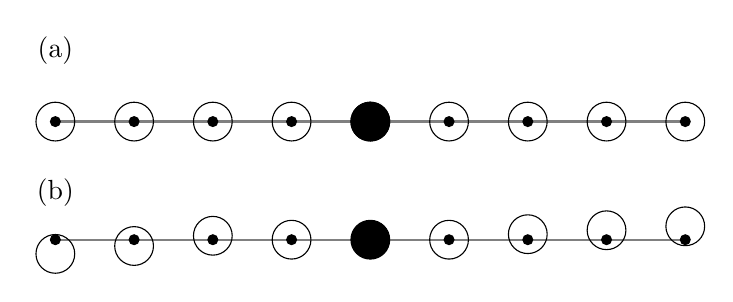
\begin{tikzpicture}
\draw[thick, gray] (0,0) -- (8,0);
\foreach \x in {0,1,2,...,8}{
\draw (\x,0) circle (7pt);
\fill (\x,0) circle (2pt);}
\draw[fill] (4,0) circle (7pt);
\draw[thick, gray] (0,-1.5) -- (8,-1.5);
\foreach \x in {0,1,2,...,8}{
\fill (\x,-1.5) circle (2pt);}
\draw (0,-1.68) circle (7pt);
\draw (1,-1.58) circle (7pt);
\draw (2,-1.45) circle (7pt);
\draw (3,-1.5) circle (7pt);
\draw[fill] (4,-1.5) circle (7pt);
\draw (5,-1.5) circle (7pt);
\draw (6,-1.43) circle (7pt);
\draw (7,-1.38) circle (7pt);
\draw (8,-1.33) circle (7pt);
\node [above] at (0,.6) {(a)};
\node [above] at (0,-1.2) {(b)};
\end{tikzpicture}%}
\caption[晶体的长程有序与液体的短程有序。]{晶体的长程有序与液体的短程有序。\label{fig-70}}
\end{figure}
液体与晶体之间的这种相似，导致出现了液体“准晶性”（quasi-crystallinity）的说法。
\pnote{“准晶性”是 20 世纪中期描述液体结构的旧术语，指液体保留局部有序。它与 20 世纪 80 年代发现的固体“准晶”是两回事——译名恰好相同，切勿混淆；今天已改用“短程有序”等统计表述。}

\stdb 那样的话，看来就可以仿照晶体来处理液体了。

\tchr 我要提醒你，不要滥用液体的准晶性概念，不要把它看得过重。第一，必须记住，液态对应着一个很宽的温度范围，不能期望液体在整个范围内的结构—动力学性质都相同（甚至近似相同）。在临界状态附近，液体显然应当失去与固体的一切相似，逐渐转变为气相。因此，液体的准晶性概念即便成立，也只是在熔点附近的某个范围内。第二，分子间相互作用的性质因液体而异。因此，准晶性概念并不是同等适用于一切液体的。例如，已经查明，水是比熔融金属更典型的准晶性液体，这解释了水的许多特殊性质（见\chap{ch-19}）。

\stdb 我现在明白了，液体中分子的热运动并没有一个简单的图像。

\tchr 完全正确。只有极端情形比较简单，中间情形总是复杂的。

\stda 物理入学考试的考纲里有关于分子动理论依据的问题。看来，应当谈谈布朗运动（Brownian motion）。

\tchr 是的，布朗运动是证实分子动理论基本原理的引人注目的实验证据。可是，你知道布朗运动究竟是什么吗？

\stda 它是分子的热运动。

\tchr 你错了；布朗运动用普通显微镜就能观察到！它是物质的个别微粒被介质分子在其热运动中不断撞击所产生的运动。从分子的观点看，这些微粒是宏观物体；但按通常的标准衡量，它们又极其微小。由于同分子的碰撞是随机的、不平衡的，布朗粒子不停地作杂乱无章的运动，从而在介质中到处移动——这种介质通常是某种液体。
\pnote{布朗运动是中国教材中分子动理论的核心实验证据（人教版选择性必修第三册第一章“分子热运动”部分），表述与教师此处完全一致：布朗运动不是分子自身的运动，而是悬浮微粒在介质分子撞击下的无规则运动，它反映了分子热运动的无规则性；微粒越小、温度越高，布朗运动越剧烈——原因正是下面的两条论证。}

\stdb 可是，为什么布朗粒子必须这么小？为什么我们观察不到尺寸可观的物质微粒（比如一杯茶里的茶叶）的布朗运动？

\begin{figure}
\centering
%\fbox{
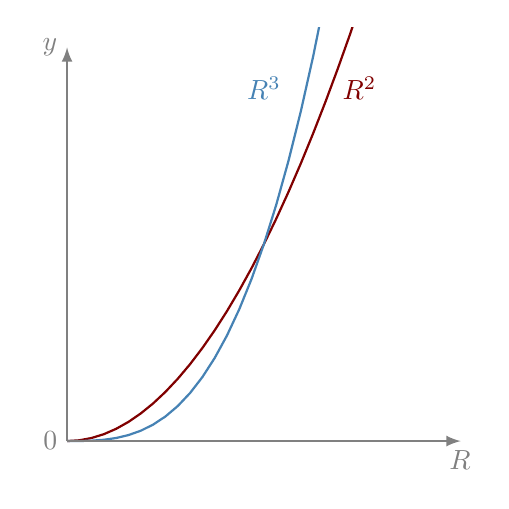
\begin{tikzpicture}[>=latex,domain=0:1.5,scale=2.5]
	%\draw[gray,step=0.2] (-5,-5) grid (5, 5);
%	\clip (-1,-1) rectangle (3, 2.1);
	\clip (-0.2,-0.2) rectangle (2.1, 2.1);
	
	\draw[thick,Maroon] plot (\x,\x*\x)	;
	\draw[thick,SteelBlue] plot (\x,\x*\x*\x);
	\node[below right,Maroon] at (1.35,1.9 ) {$R^{2}$};
	\node[below,SteelBlue] at (1,1.9) {$R^{3}$};
		
	\draw[thick, ->, gray] (0,0) -- (2,0);
	\draw[thick, ->, gray] (0,0) -- (0,2);
	\node [left,gray] at (0,2) {$y$};
	\node [below left,gray] at (2.1,0) {$R$};
	\node [left,gray] at (0,0) {0};

\end{tikzpicture}%}
\caption[表面积与体积关系的效应。]{表面积与体积关系的效应。\label{fig-71}}
\end{figure}


\tchr 这有两个原因。第一，分子同微粒表面的碰撞次数与表面积成正比，而微粒的质量与它的体积成正比。于是，随着微粒尺寸 $R$ 的增大，分子与其表面的碰撞次数按 $\hlred{R^{2}}$ 成比例地增加，而碰撞所要挪动的微粒质量则按 $\hlblue{R^{3}}$ 成比例地增加。因此，微粒越大，分子越难推动它们。为使这一点更清楚，我在\figr{fig-71} 中画了两条曲线：$y=\hlred{R^{2}}$ 和 $y=\hlblue{R^{3}}$。容易看出，$R$ 值小时平方关系占上风，$R$ 值大时立方关系占上风。这就是说，$R$ 值小时表面效应占优势，$R$ 值大时体积效应占优势。

第二，布朗粒子必须非常小，因为它同分子的碰撞是不平衡的，也就是说，单位时间内从左边和从右边受到的碰撞次数应当相差显著。而微粒的表面越小，这个碰撞次数之差与总碰撞次数之比就越大。
\pnote{第二条理由即统计涨落：粒子表面越小，单位时间内的碰撞总数 $N$ 越少，而撞击不平衡的相对偏差量级为 $1/\sqrt{N}$，故小粒子的不平衡撞击相对越显著。\figr{fig-71} 中两条曲线按无量纲数值画出（交点在 $R=1$），只用于比较平方律与立方律增长的快慢；实际估算只保留比例关系：碰撞数 $\propto R^{2}$，质量 $\propto R^{3}$。}

\stda 我们还应当知道哪些证实分子动理论的事实呢？

\tchr 对分子动理论最好的证实，是它成功地应用于解释大量物理现象。例如，可以解释气体对盛它的容器器壁的压强。压强 $p$ 是作用在器壁单位面积上的力 $F$ 的法向分量。由于
\begin{equation}
F=m \left( \frac{\Delta v}{\Delta t} \right) =  \frac{\Delta (mv)}{\Delta t}
\label{eq-100}
\end{equation}
为求压强，我们必须确定气体分子撞击器壁时在单位时间内传给器壁单位面积的动量。

设质量为 $m$ 的一个分子以速度 $v$ 垂直于器壁飞行。与器壁发生弹性碰撞后，分子反转飞行方向，以速度 $v$ 离开器壁飞走。分子动量的改变等于 $\Delta (mv)=m \Delta v=2mv$。这份动量传给了器壁。为简单起见，我们将假设气体中所有分子都具有同样的速度 $v$，且沿三条坐标轴的正、负两个方向共有六种运动方向（设器壁垂直于其中一条轴）。其次，要考虑到：单位时间内能到达器壁的，只是那些离器壁的距离在 $v$ 以内、且速度指向器壁的分子。既然气体的单位体积内含有 $N/V$ 个分子，那么单位时间内就有 $\dfrac{1}{6}\left(\dfrac{N}{V} \right)v$ 个分子打到器壁的单位面积上。由于其中每个分子传递动量 $2mv$，这些撞击的结果，是器壁单位面积获得大小为 $2mv \dfrac{1}{6}\left(\dfrac{N}{V} \right)v$ 的动量。根据式~\eqref{eq-100}，这就是所求的压强 $p$。于是
\begin{equation}%
p= \frac{2}{3}\frac{N}{V} \frac{mv^{2}}{2}
\label{eq-101}
\end{equation}
根据式~\eqref{eq-98}，可以把分子的能量 $\dfrac{mv^{2}}{2}$ 换成量 $\dfrac{3}{2} kT$［就分子的平动而言，式~\eqref{eq-98} 对具有任意数目原子的分子都成立］。此后，式~\eqref{eq-101} 可以改写为
\begin{equation}%
pV=NkT
\label{eq-102}
\end{equation}
注意，这个结果是在对问题作了相当大的简化之后得到的（例如，假设了气体分子都以同一速度飞行）。然而，理论表明，这个结果与严格处理所得的结果完全一致。

式~\eqref{eq-102} 得到直接测量的漂亮证实。这是对推导式~\eqref{eq-102} 时所用分子动理论概念的正确性的很好证明。
\pnote{“六分之一”模型与中国教材对压强的微观解释一致（人教版选择性必修第三册第二章）；式~\eqref{eq-102} 为气体方程的分子数形式（$N/V$ 为分子数密度），与 $pV=nRT$ 等价，比较得 $R=N_{A}k$。}

现在，让我们在分子动理论观念的基础上讨论液体的蒸发和沸腾现象。\hlred{你怎样解释蒸发现象？}

\stda 液体里那些最快的分子克服其余分子的吸引，飞出液面。

\tchr 什么因素会加剧蒸发？

\stda 第一是增大液体的自由表面，第二是给液体加热。

\tchr 应当记住，蒸发是双向的过程：一部分分子离开液体，另一部分分子同时返回液体。离开的分子数与返回的分子数之比越大，蒸发就越有效。加热液体和增大它的自由表面会加剧分子从液体中逸出。同时，也可以采取措施减少分子返回液体。例如，若有风沿液面吹过，刚逸出的分子就被带走，从而减小了它们返回的概率。湿衣服在风里干得快，道理就在这里。

如果分子从液体中逸出与它们返回液体相互抵偿，就会建立起动态平衡，液体上方的蒸汽就成为饱和汽（saturated vapour）。在某些场合，减缓蒸发过程是有益的。例如，面包中的水分迅速蒸发是我们所不希望的。为了防止面包很快变干，要把它保存在密闭的容器里（面包盒、塑料袋）。这就阻碍了蒸发出来的分子散失，在面包表面上方形成一层饱和汽，阻止面包中的水分继续蒸发。

现在，请你来解释沸腾过程。

\stda 沸腾过程同蒸发是一样的，只是进行得更剧烈。

\tchr 我一点也不喜欢你这个沸腾过程的定义。我要指出，许多考生并不理解这个过程的实质。加热液体时，溶解在其中的气体的溶解度减小，结果液体中（容器底和壁上）形成了气泡。蒸发在这些气泡内进行，气泡里充满饱和汽，其压强随液体温度的升高而增大。在某一温度下，气泡内饱和汽的压强变得与外部作用在气泡上的压强相等（这个压强等于大气压强加上气泡上方水层的压强）。从这个时刻起，气泡迅速上升到液面，液体就沸腾了。如你所见，液体的沸腾与蒸发有本质的区别。注意，\hlblue{蒸发在任何温度下都能发生，而沸腾则在确定的温度——沸点——下发生。}我还要提醒你：\hlblue{沸腾过程一经开始，无论我们继续加热多久，液体的温度都不可能再升高。温度将保持在沸点，直到全部液体蒸发完为止。}
\pnote{“气压减小，沸点降低”自初中物理（人教版八年级上册第三章《物态变化》“汽化和液化”）即有交代，高压锅与低压沸腾演示都基于此。教师所述“气泡内饱和汽压等于外部压强即沸腾”与现行教材的沸腾条件一致；下文抽气一题正是“降低外压强使室温的水沸腾”的经典演示。}

由上可见，外部压强减小时，液体的沸点降低。就此我们来看下面这个问题。\hlred{烧瓶里盛有少量室温的水。我们开始用真空泵从烧瓶中抽出水上方的空气。水会发生什么情况？}

\stda 随着空气被抽走，瓶内压强降低，沸点随之降低。当沸点降到室温时，水就开始沸腾。

\tchr 水有没有可能不沸腾，反而结冰呢？

\stda 我说不上来。我想不会。

\tchr 这完全取决于从瓶中抽气的快慢。如果这个过程足够慢，水迟早应当开始沸腾。但如果抽气非常快，水反而应当结冰。由于空气（连同水蒸气）被抽走，蒸发过程加剧。既然蒸发时从水中逃逸的是能量较大的分子，剩下的水就会被冷却。若抽气缓慢，冷却效应会被从外界传入的热量补偿，结果水温保持不变。若抽气非常快，水的冷却来不及由外界流入的热量补偿，水温就开始下降。而这一旦发生，沸腾的可能性也随之减小。从瓶中继续快速抽气，将使水温降到冰点，尚未蒸发的余下的水就变成冰。

\end{dialogue}


\cleardoublepage

% NEWTERMS: molecular-kinetic theory of matter | （物质的）分子动理论 | 章名术语；人教版选择性必修第三册第一章《分子动理论》；首现括注英文
% NEWTERMS: gram-molecule | 克分子 | 旧术语，即 1 mol；现行课程用摩尔，见评注
% NEWTERMS: gram-atom | 克原子 | 同克分子，按原子计
% NEWTERMS: Avogadro's number | 阿伏加德罗常数 | 人教版拼法“阿伏加德罗”（不作“阿伏伽德罗”）；原书称 number（数），现行定义值见评注
% NEWTERMS: Boltzmann's constant | 玻耳兹曼常量 | 名词委《物理学名词》作“玻耳兹曼”；常见异写“玻尔兹曼”；CGS→SI 换算见评注
% NEWTERMS: absolute temperature | 绝对温度 | 即现行教材的热力学温度 T（单位 K）
% NEWTERMS: chaotic thermal motion | 无规则热运动 | 人教版表述“无规则”（不用“杂乱无章”作术语）
% NEWTERMS: internal energy | 内能 | 人教版选择性必修第三册第一章第 4 节；式 (99) 之 U
% NEWTERMS: crystal lattice | 晶格 | 结点＝分子平衡位置；亦译“晶体点阵”
% NEWTERMS: lattice points | （晶格）结点 | |
% NEWTERMS: binding energy | 结合能 | 分子内原子的／分子在晶格中的
% NEWTERMS: bound state | 束缚态 | 大学词汇，评注中类比束缚系统
% NEWTERMS: short-range order | 短程有序 | 液体结构术语，X 射线散射确立
% NEWTERMS: long-range order | 长程有序 | 晶体有序
% NEWTERMS: quasi-crystallinity | 准晶性 | 旧术语；勿与“准晶”（quasicrystal）混淆，见评注
% NEWTERMS: jump-diffusion model | 跳跃扩散模型 | 液体分子运动模型之一
% NEWTERMS: continuous-diffusion model | 连续扩散模型 | 同上
% NEWTERMS: coefficient of volume expansion | 体胀系数 | 亦称体膨胀系数
% NEWTERMS: heat of fusion / heat of vaporization | 熔化热／汽化热 | 人教版同名
% NEWTERMS: critical state | 临界状态 | |
% NEWTERMS: saturated vapour | 饱和汽 | 人教版用“汽”（不用“气”）
% NEWTERMS: dynamic equilibrium | 动态平衡 | 蒸发与返回抵偿的平衡
% NEWTERMS: Brownian motion | 布朗运动 | 人教版选择性必修第三册第一章；非分子自身的运动
% NEWTERMS: Brownian particle | 布朗粒子 | |
% NEWTERMS: boiling point | 沸点 | 随外压强降低而降低
% NEWTERMS: molecular weight / atomic weight | 分子量／原子量 | 现行课程称相对分子质量／相对原子质量，见评注
% NEWTERMS: translatory / rotary / vibratory motion | 平动／转动／振动 | 平动沿第 2 章 motion of translation 译名
% NEWTERMS: monoatomic molecule | 单原子分子 | |
